
\title{New figures from IBM analysis, final chapter}
\author{
        Chris McWilliams*, Alan Champneys, Miguel Lurgi,\\ Jose Montoya, Daniel Montoya \\ \\
				*Bristol Centre for Complexity Sciences, University of Bristol.\\
                chris.mcwilliams@bristol.ac.uk\\
}
\date{\today}

\documentclass[12pt]{article}
\usepackage{mathtools}
\usepackage{amsmath}
\usepackage{amssymb}
\usepackage{appendix}
\usepackage{graphicx}
\usepackage{caption}
\usepackage{subcaption}
\usepackage{rotating}
%\usepackage{subfig}
\usepackage[font={small,it}]{caption}
\usepackage[font={small,it}]{subcaption}
\usepackage{todo}
\setlength\parindent{0pt}
\setlength{\parskip}{10pt plus 1pt minus 1pt}

\newcommand{\mbeq}{\overset{!}{=}}

\begin{document}

\section{2 species, no habitat loss.}

These figures show results from fitting GLV model to 2 species IBM simulations.

\begin{figure}[b]
	\centering
	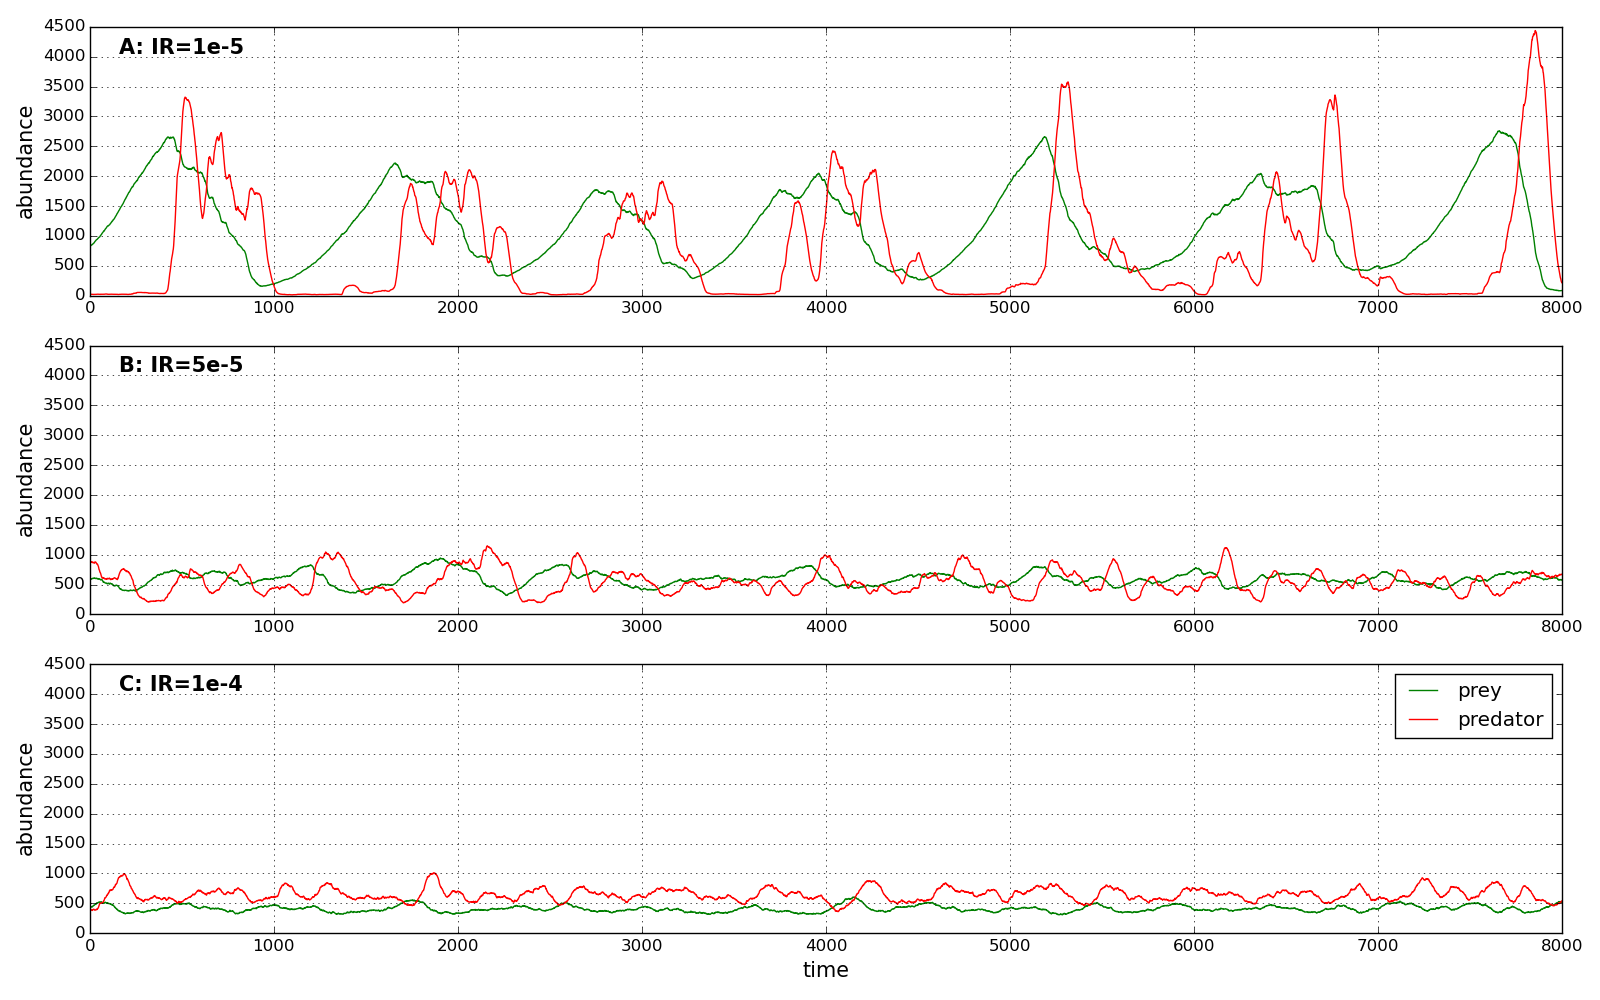
\includegraphics[width=\textwidth]{{{2species/example_dynamics_2sp_nohl}}}
	\label{fig:example_dynamics}
	\caption{Example dynamics of three simulation runs with different IR. Initial transience removed.}
\end{figure}

\begin{figure}[b]
	\centering
	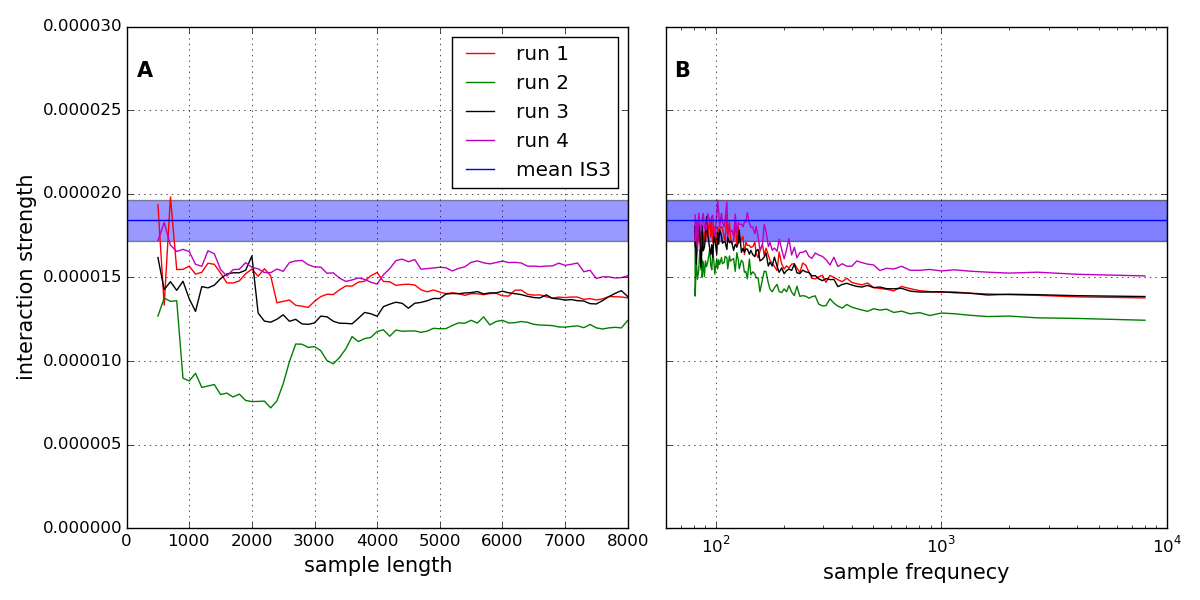
\includegraphics[width=\textwidth]{{{2species/convergence_highIR}}}
	\label{fig:conv_high}
	\caption{Convergence of estimator $\hat{J}_{01}$. High IR (0.0001).}
\end{figure}

\begin{figure}
	\centering
	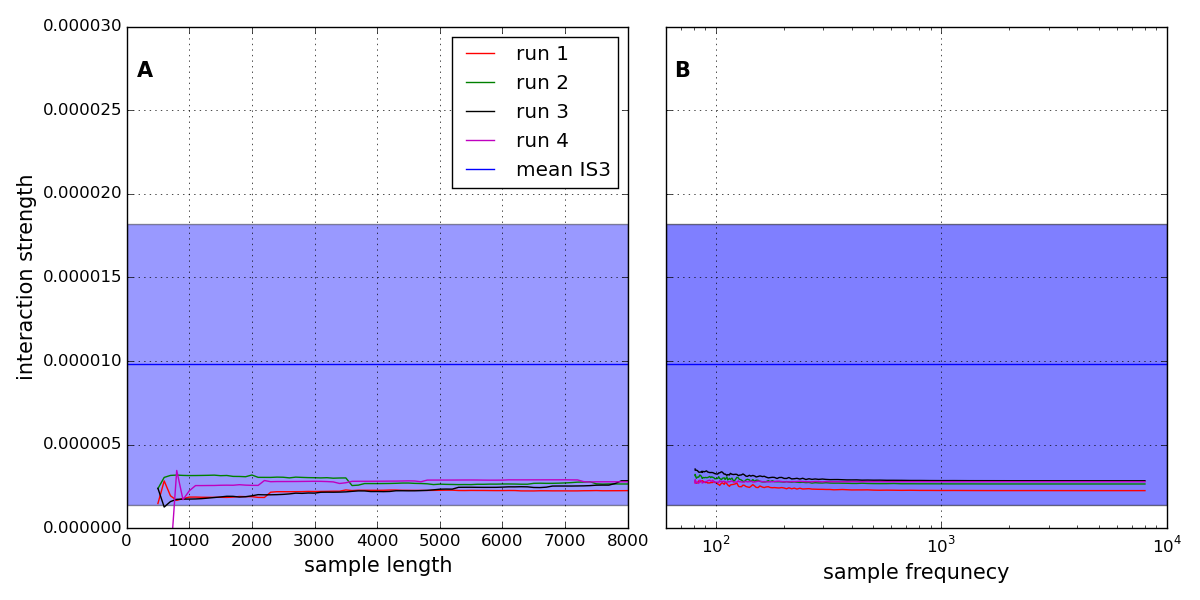
\includegraphics[width=\textwidth]{{{2species/convergence_lowIR}}}
	\label{fig:conv_low}
	\caption{Convergence of estimator $\hat{J}_{01}$. Low IR (0.00001).}
\end{figure}


\begin{figure}
	\centering
	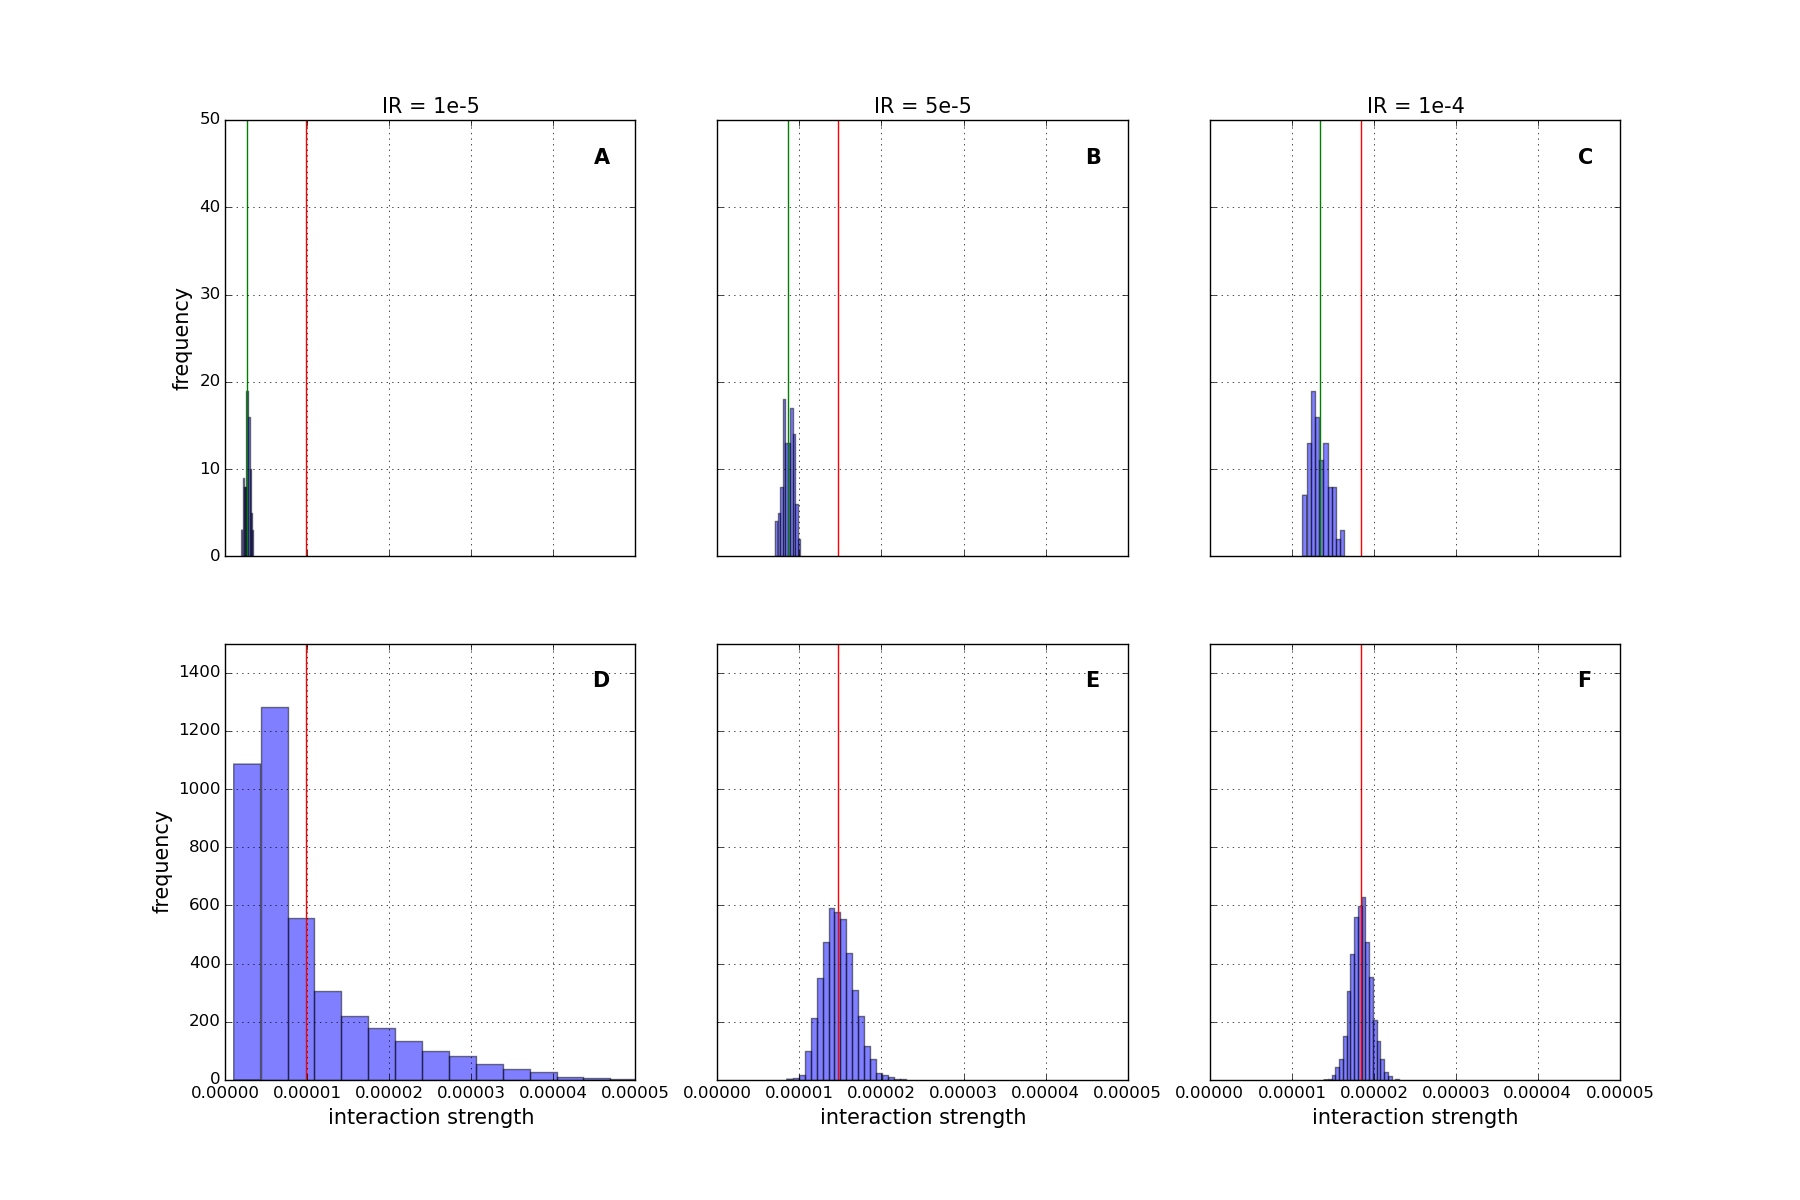
\includegraphics[width=\textwidth]{{{2species/J01_ensemble_estimates_2sp_nohl}}}
	\label{fig:ensemble_J01}
	\caption{Distribution of prey interaction strengths for three ensembles of simulations at different IR. Top row: estimates produced by fitting GLV model. Bottom row: Estimates produced by counting number of prey consumed.}
\end{figure}


\begin{figure}
	\centering
	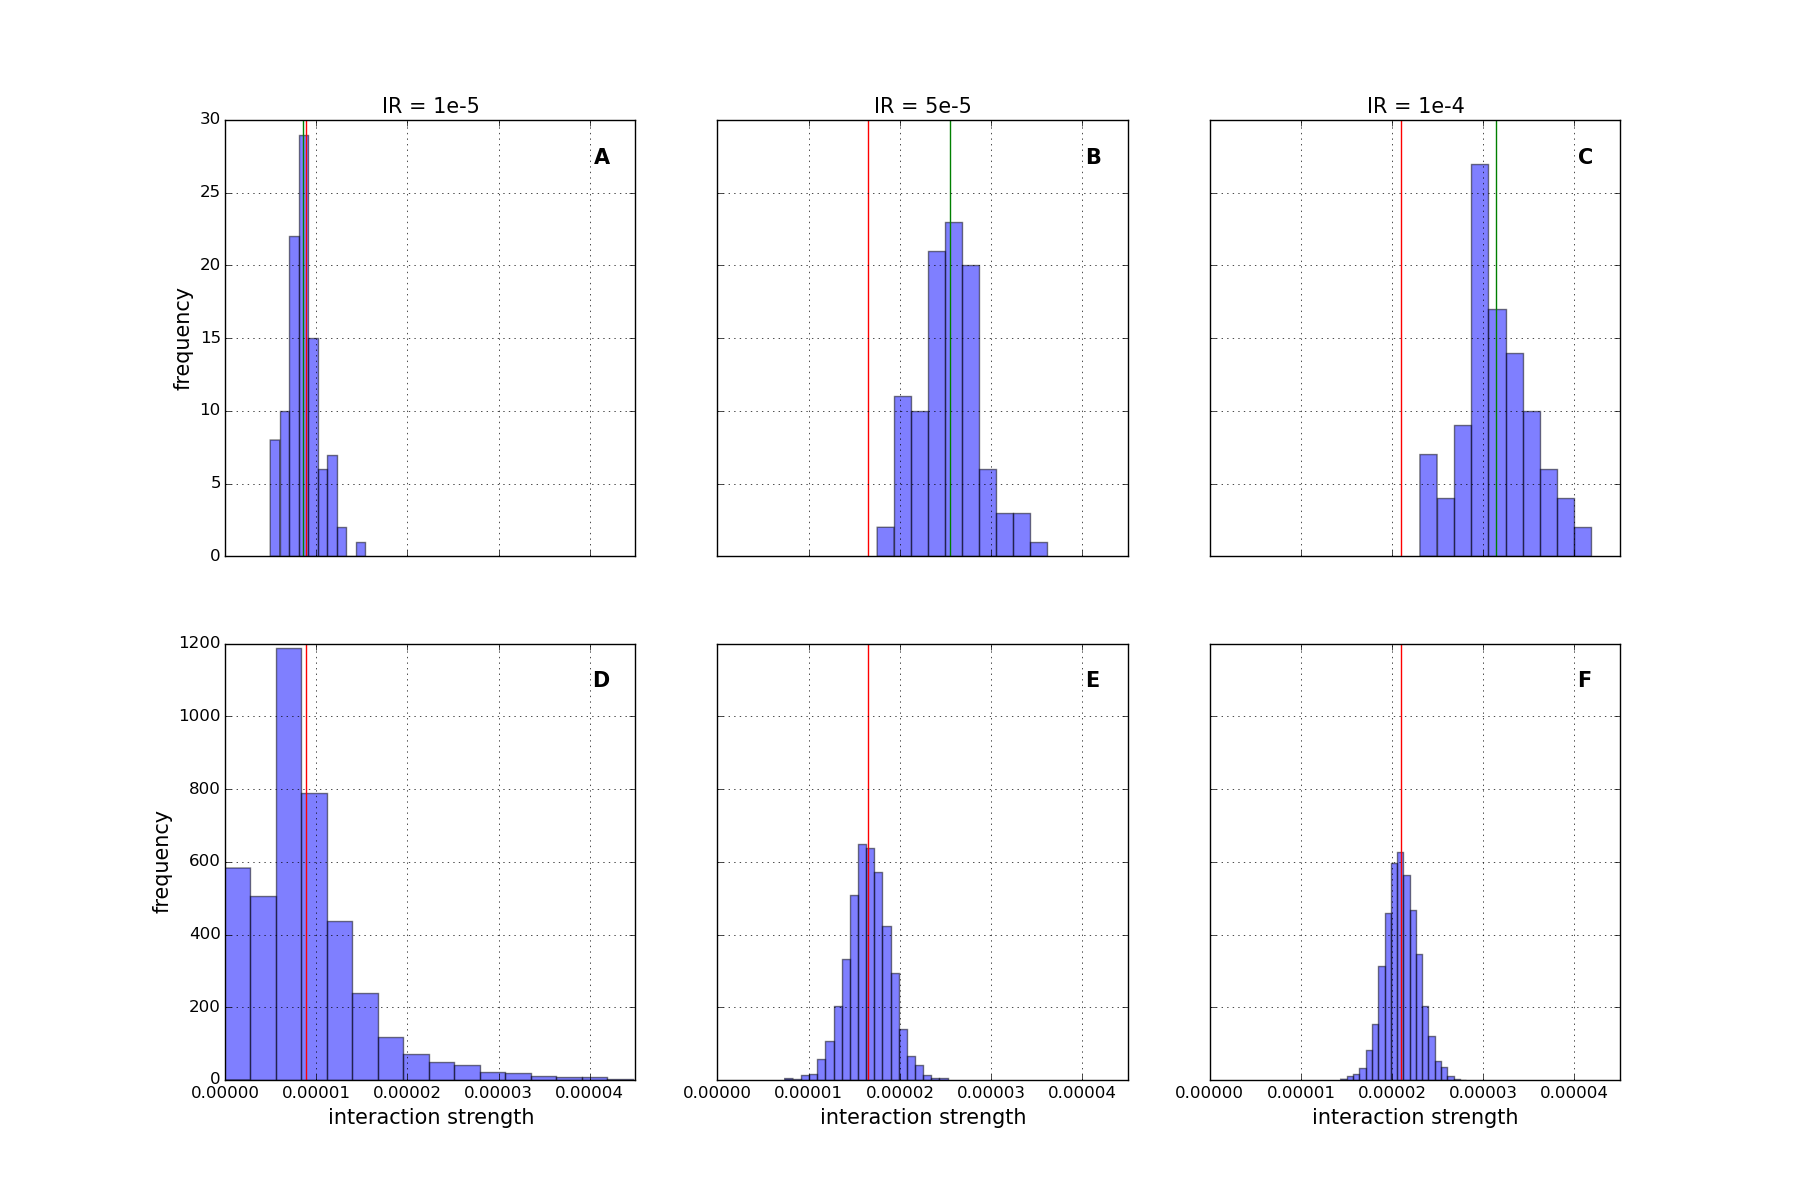
\includegraphics[width=\textwidth]{{{2species/J10_ensemble_estimates_2sp_nohl}}}
	\label{fig:ensemble_J10}
	\caption{Distribution of predator interaction strengths for three ensembles of simulations at different IR. Top row: estimates produced by fitting GLV model. Bottom row: Estimates produced by counting number of predators born.}
\end{figure}


\begin{figure}
	\centering
	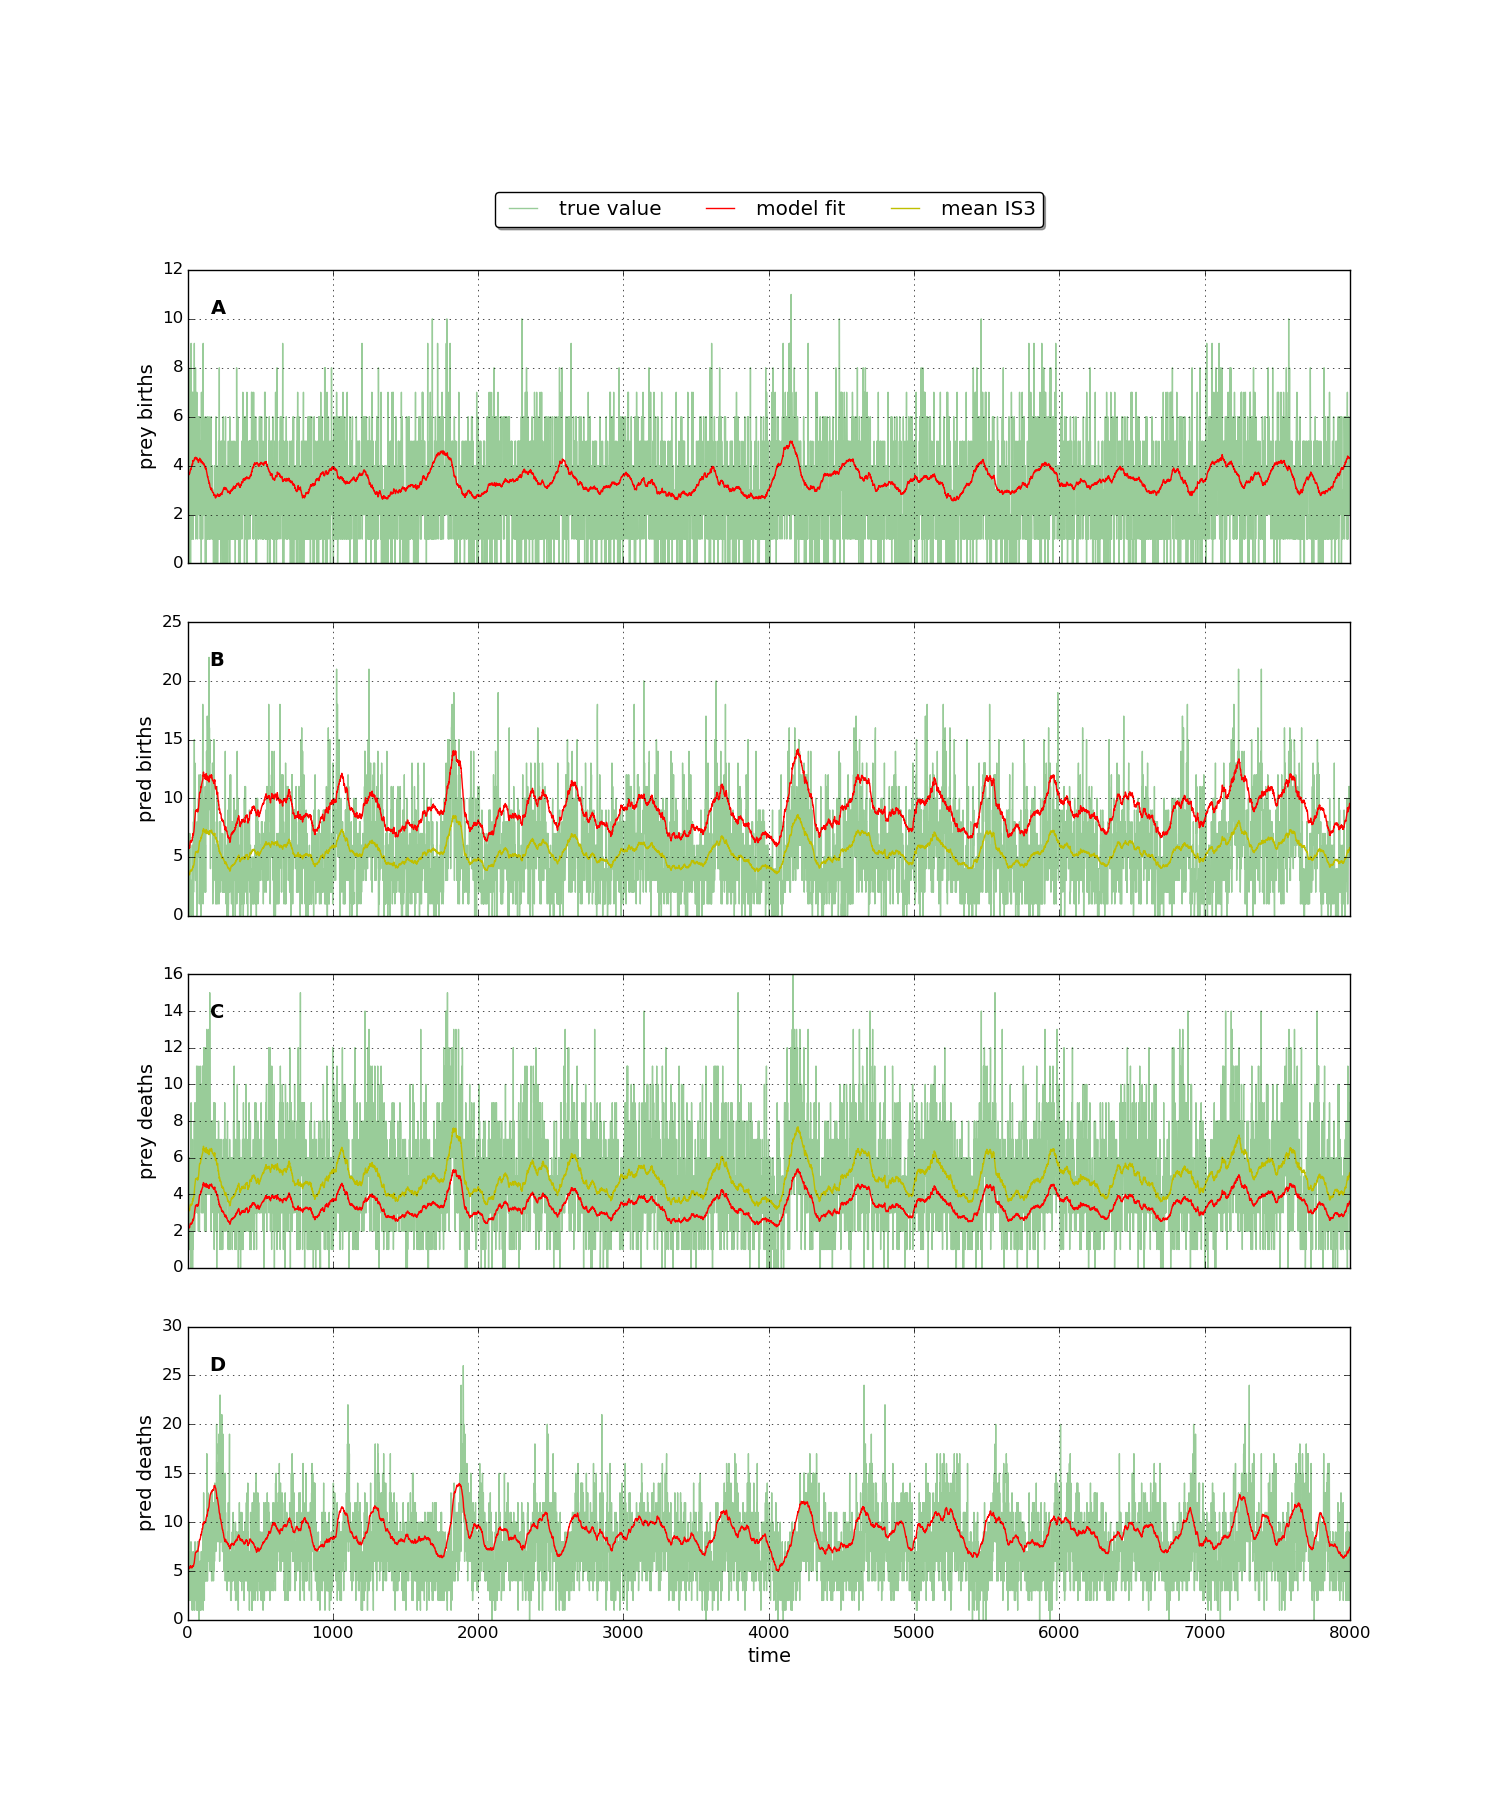
\includegraphics[width=\textwidth]{{{2species/back_check_highIR_4463199_4}}}
	\label{fig:backcheck_high}
	\caption{Comparing actual births and death rates to those predicted by the fitted model. Single simulation run, high IR (0.0001)}
\end{figure}


\begin{figure}
	\centering
	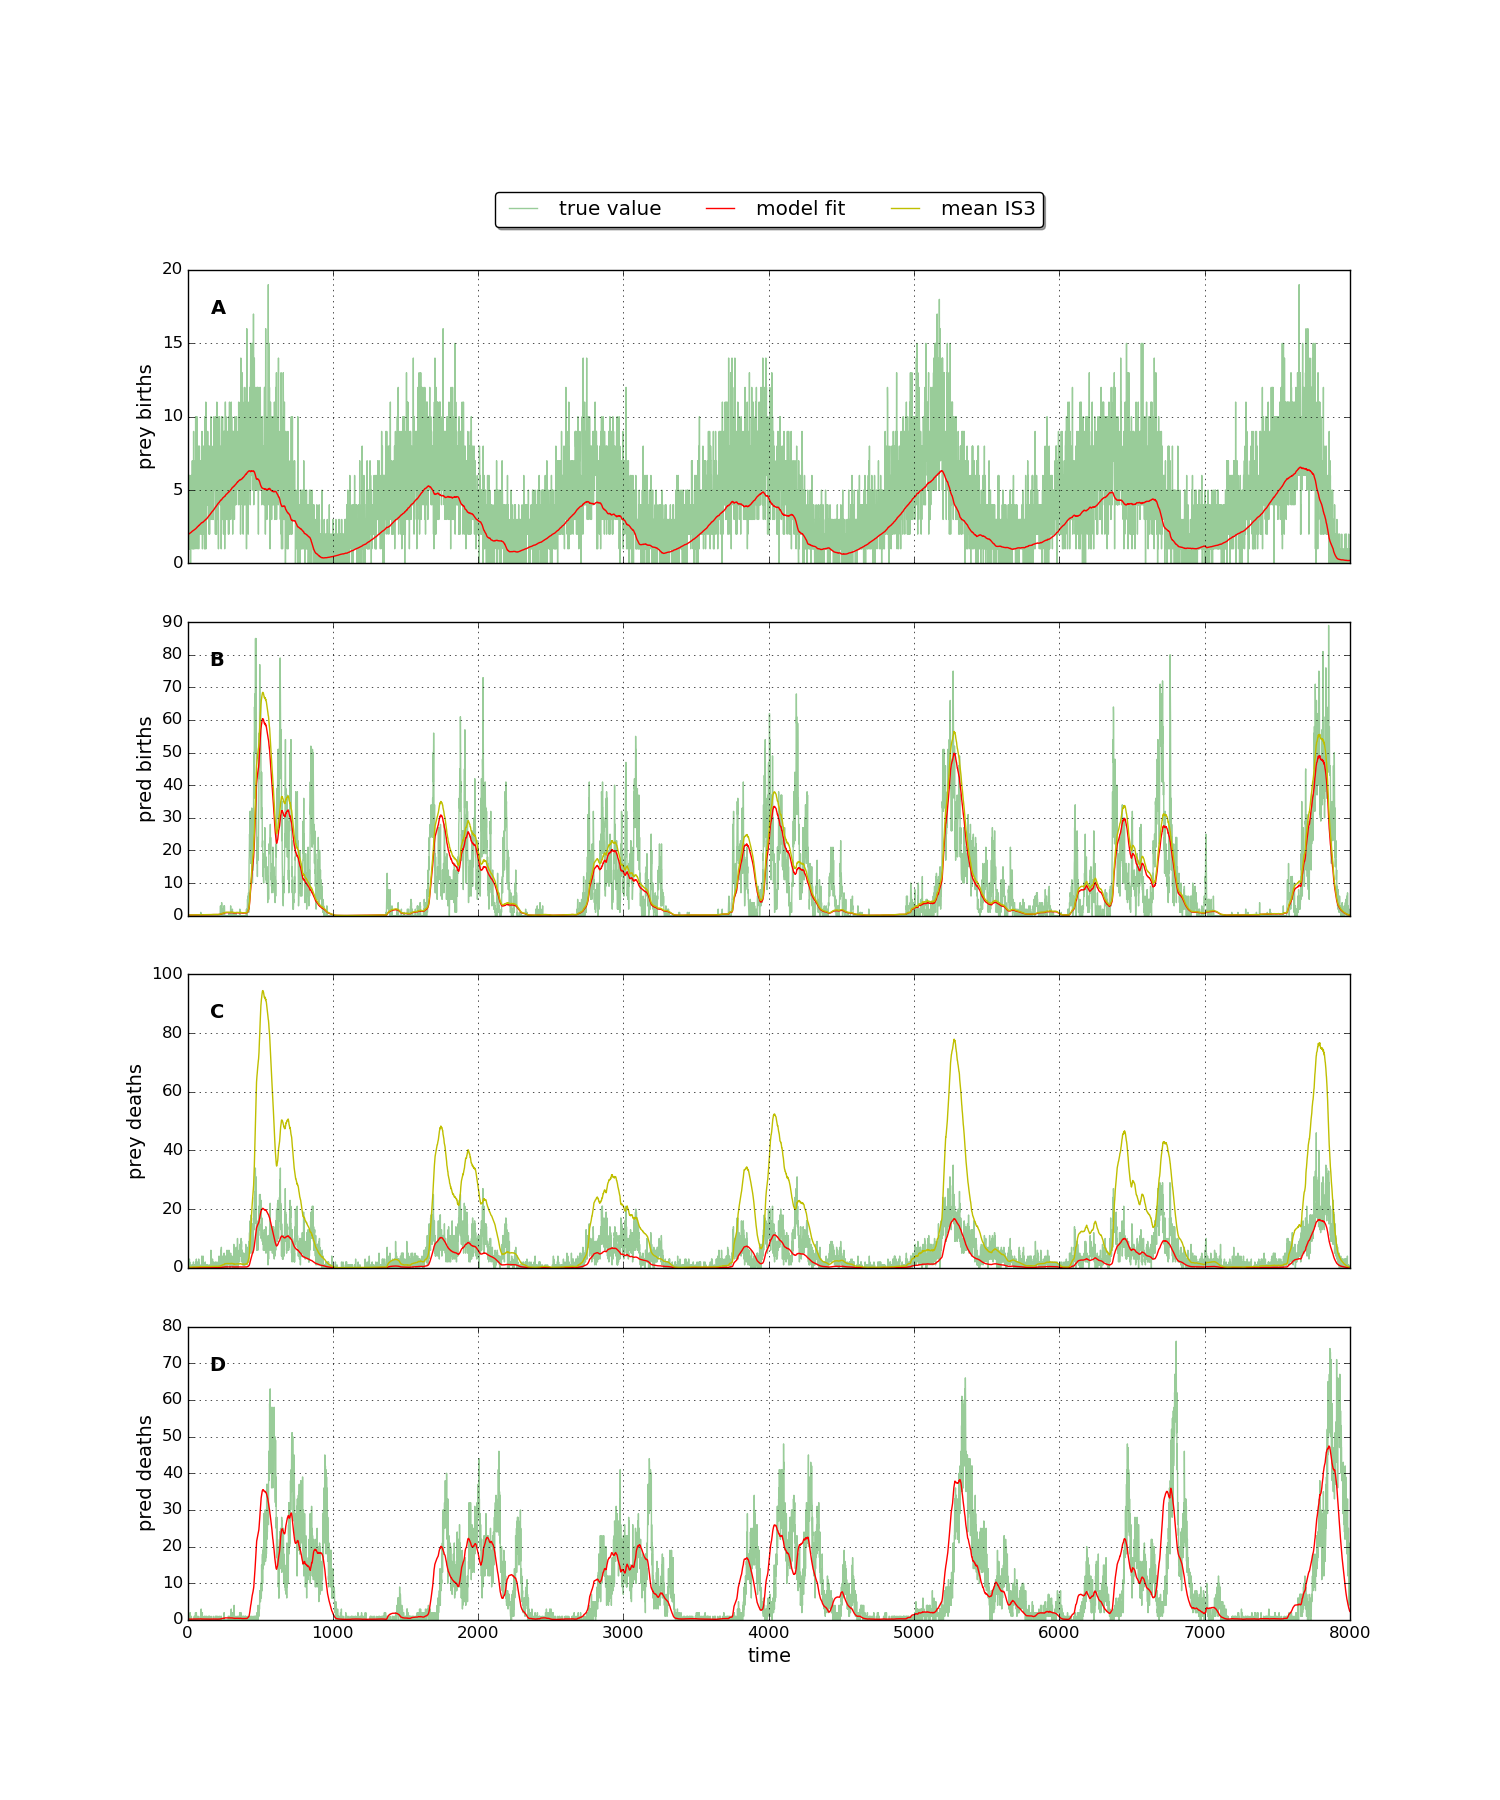
\includegraphics[width=\textwidth]{{{2species/back_check_lowIR_4463195_3}}}
	\label{fig:backcheck_low}
	\caption{Comparing actual births and death rates to those predicted by the fitted model. Single simulation run, low IR (0.00001)}
\end{figure}


\clearpage
\section{2 species, with habitat loss.}

\begin{figure}[b]
	\centering
	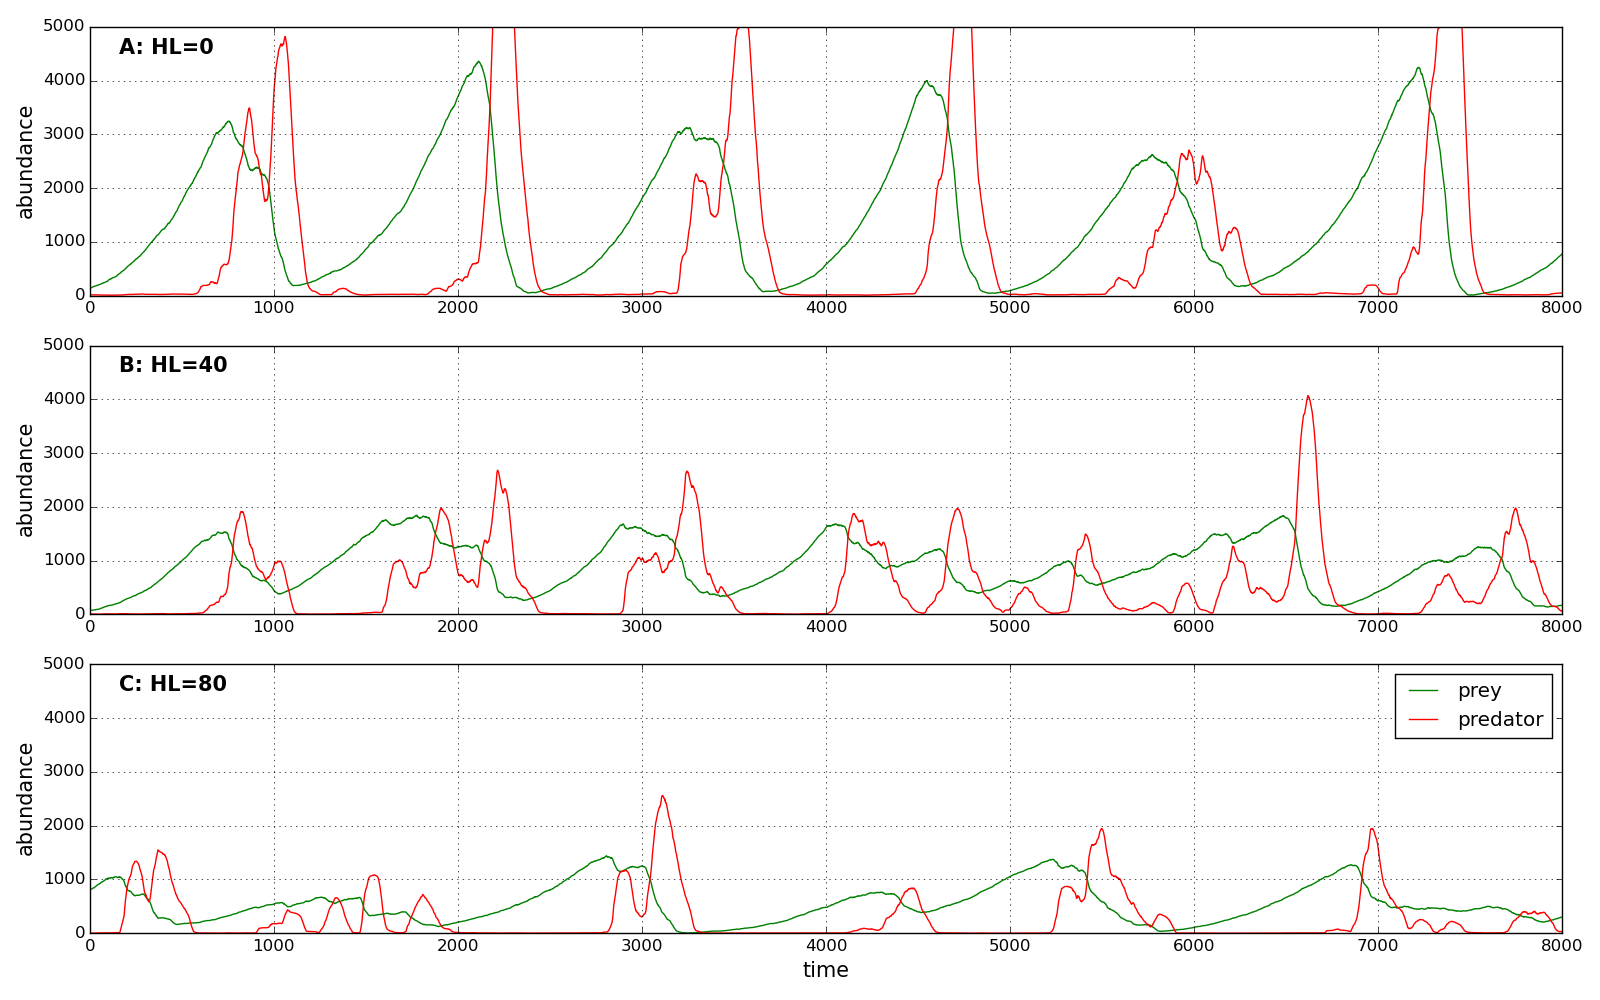
\includegraphics[width=\textwidth]{{{2species/example_dynamics_2sp_contiguous}}}
	\label{fig:example_dynamics_contig}
	\caption{Example dynamics of three simulation runs with different levels of contiguous HL. Initial transience removed.}
\end{figure}

\begin{figure}[b]
	\centering
	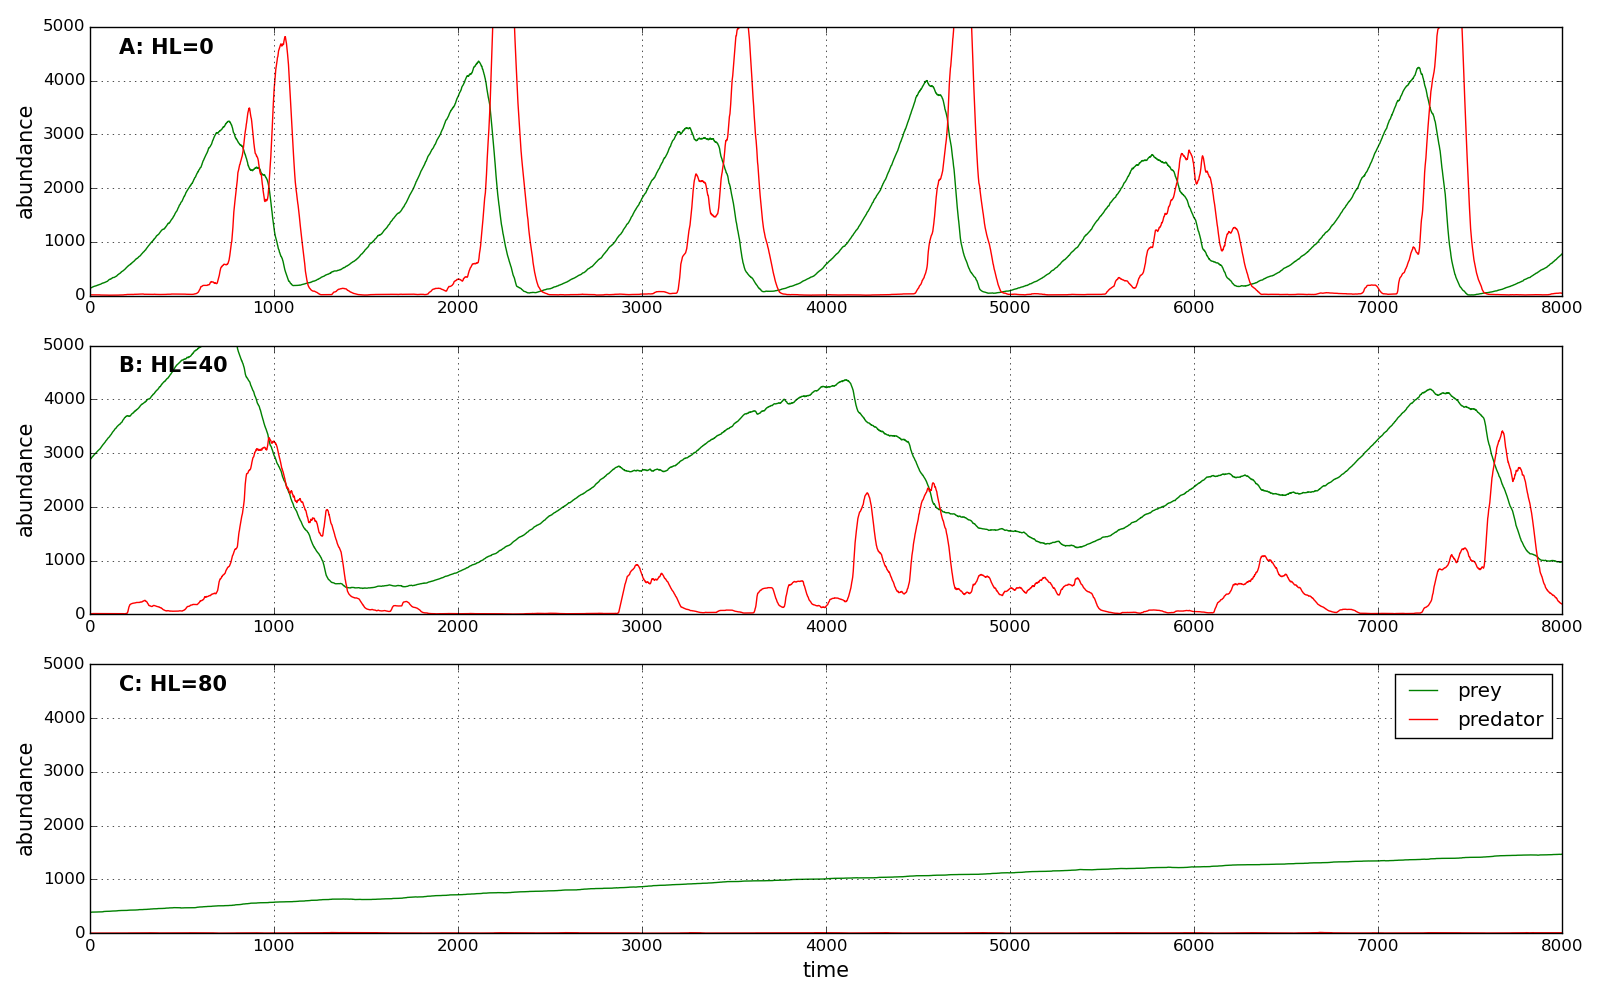
\includegraphics[width=\textwidth]{{{2species/example_dynamics_2sp_random}}}
	\label{fig:example_dynamics_rand}
	\caption{Example dynamics of three simulation runs with different levels of random HL. Initial transience removed.}
	\end{figure}



\end{document}


